\documentclass{beamer}
\usepackage{tikz}
\usepackage{graphicx}

\newcommand{\drawperiod}[6]{%
  % Arguments: start year, start month, end year, end month, fill color, image
  \pgfmathsetmacro{\startx}{1.25*#1 + 1.25*(#2-1)/12 - 1.25*2016} % Calculate start position based on year and month
  \pgfmathsetmacro{\endx}{1.25*#3 + 1.25*(#4-1)/12 - 1.25*2016}   % Calculate end position based on year and month
  \draw[fill=#5] (\startx,0.4) rectangle (\endx,1.2); % Draw rectangle with reduced height
  \node at ({(\startx+\endx)/2}, 0.8) {\includegraphics[height=1cm]{#6}}; % Center the image
  % draw lines to the timeline - isprekidano
  \draw [dashed] (\startx,0.4) -- (\startx,0);
  \draw [dashed] (\endx,0.4) -- (\endx,0);
}

\newcommand{\drawperiodabove}[6]{%
  % Arguments: start year, start month, end year, end month, fill color, image
  \pgfmathsetmacro{\startx}{1.25*#1 + 1.25*(#2-1)/12 - 1.25*2016} % Calculate start position based on year and month
  \pgfmathsetmacro{\endx}{1.25*#3 + 1.25*(#4-1)/12 - 1.25*2016}   % Calculate end position based on year and month
  \draw[fill=#5] (\startx,2.0) rectangle (\endx,2.8); % Draw rectangle with reduced height
  \node at ({(\startx+\endx)/2}, 2.4) {\includegraphics[height=1cm]{#6}}; % Center the image
  % draw lines to the timeline - isprekidano
  \draw [dashed] (\startx,2.0) -- (\startx,0);
  \draw [dashed] (\endx,2.0) -- (\endx,0);
}


\newcommand{\drawperiodbelow}[6]{%
  % Arguments: start year, start month, end year, end month, fill color, image
  \pgfmathsetmacro{\startx}{1.25*#1 + 1.25*(#2-1)/12 - 1.25*2016} % Calculate start position based on year and month
  \pgfmathsetmacro{\endx}{1.25*#3 + 1.25*(#4-1)/12 - 1.25*2016}   % Calculate end position based on year and month
  \draw[fill=#5] (\startx,-1.0) rectangle (\endx,-1.8); % Draw rectangle with reduced height
  \node at ({(\startx+\endx)/2}, -1.4) {\includegraphics[height=0.5cm]{#6}}; % Center the image
  % draw lines to the timeline
  \draw [dashed] (\startx,-1.2) -- (\startx,0);
  \draw [dashed] (\endx,-1.2) -- (\endx,0);
}

\newcommand{\drawperiodbelowbelow}[6]{%
  % Arguments: start year, start month, end year, end month, fill color, image
  \pgfmathsetmacro{\startx}{1.25*#1 + 1.25*(#2-1)/12 - 1.25*2016} % Calculate start position based on year and month
  \pgfmathsetmacro{\endx}{1.25*#3 + 1.25*(#4-1)/12 - 1.25*2016}   % Calculate end position based on year and month
  \draw[fill=#5] (\startx,-2.0) rectangle (\endx,-2.8); % Draw rectangle with reduced height
  \node at ({(\startx+\endx)/2}, -2.4) {\includegraphics[height=0.5cm]{#6}}; % Center the image
  % draw lines to the timeline
  \draw [dashed] (\startx,-2.2) -- (\startx,0);
  \draw [dashed] (\endx,-2.2) -- (\endx,0);
}

\begin{document}

\begin{frame}{Timeline}

\begin{tikzpicture}

  % Draw the timeline
  \draw[thick] (0,0) -- (11.25,0);

  % Add year labels
  \foreach \x/\year in {0/2016, 1.25/2017, 2.5/2018, 3.75/2019, 5/2020, 6.25/2021, 7.5/2022, 8.75/2023, 10/2024} {
    \draw (\x,0.1) -- (\x,-0.1);
    % centered text
    \node[below] at (\x,-0.2) {\year};
  }

  % Draw periods using the \drawperiod command (start year, start month, end year, end month, color, image path)
  \drawperiod{2017}{9}{2018}{8}{white}{./upwork.png} 
  \drawperiod{2018}{12}{2022}{1}{white}{./conti.png} 
  \drawperiod{2022}{3}{2024}{5}{white}{./ntnx.png}  
  \drawperiodabove{2017}{1}{2024}{12}{white}{./petnica.png}  
  \drawperiodbelow{2016}{9}{2021}{1}{white}{./ftn.png} 
  \drawperiodbelow{2021}{10}{2024}{9}{white}{./pmf.png} 


\end{tikzpicture}

\end{frame}

\begin{frame}
  \frametitle{Projekti}
  \begin{tabular}{r|p{8cm}}


    %------------------------------------------------
    
    FluidSim & Fluid simulation based on solving Navier-Stokes equations \\
    Height3D & OOP framework made in C++ for making 3D apps using OpenGL. \\
    PageProc & Document layout analysis. Uses xy-cuts algorithm and various heuristics to classify elements on page.  \\ 
    Osmium & An attempt to make open source version of Wolfram language with compatible API. \\
    DistTranscode & Distributed FFmpeg (video decoding/encoding and filtering). \\
    CoNAL & Computing Node Abstraction Layer: framework for building distributed applications  \\
    CloudPost & Platform for making and deploying cloud-based applications which is vendor-agnostic \\
    \end{tabular}
    
  

\end{frame}

\begin{frame}
  \frametitle{Oblasti interesovanja}
  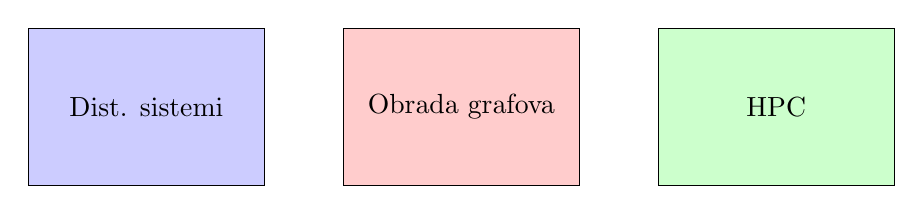
\begin{tikzpicture}
    % 4 rectangles where text is wrapped
    \draw[fill=blue!20] (0,0) rectangle (3,2) node[pos=.5] {Dist. sistemi};
    \draw[fill=red!20] (4,0) rectangle (7,2) node[pos=.5] {Obrada grafova};
    \draw[fill=green!20] (8,0) rectangle (11,2) node[pos=.5] {HPC};
  \end{tikzpicture}

  

\end{frame}

\end{document}
